\documentclass[a4paper,1pt]{article}

\usepackage[french]{babel}
\usepackage[T1]{fontenc}
\usepackage[utf8]{inputenc}
\usepackage{lmodern}
\usepackage{microtype}
\usepackage{hyperref}
\usepackage{amsmath}
\usepackage{graphicx}

\graphicspath{{/home/grybouilli/TIPE/schema/}}

\title{TIPE 2020/2021 : \\ Débris Spatiaux}
\date{12 octobre 2020}

\begin{document}
\maketitle

\section*{Objectifs}
\begin{itemize}
    \item Recherches : 
    \begin{itemize}
        \item Moment magnétique
        \item Interactions entre dipôles magnétiques
        \item Paramagnétisme
        \item Composition des satellites pour capter ce qui va réagir
    \end{itemize}
    \item Ce qu'on trouve:
    \begin{itemize}
        \item  Compo des satellites ( en tout cas à la NASA ):\\
        \url{https://www.nasa.gov/centers/johnson/pdf/584729main_Wings-ch4c-pgs200-225.pdf}\\
        $\rightarrow$ Utilisation d'alliages Li-Al et Li paramagnétique.
        \item Les Wiki :\\
        \url{https://fr.wikipedia.org/wiki/Moment_magn%C3%A9tique}
    \end{itemize}
       
\end{itemize}

\section*{Cours sur le solénoide}
On considère un solénoide de longueur $L$ de $N$ spires. On note $n$ le nombre de spires par unité de longueur:
$$n= \frac{N}{L}$$
Pour une petite longueur d$z$, on note aussi:
$$N'=n\mathrm{d}z$$
\\
\textbf{Champ élémentaire créé sur le point M}
\begin{figure}[h]
    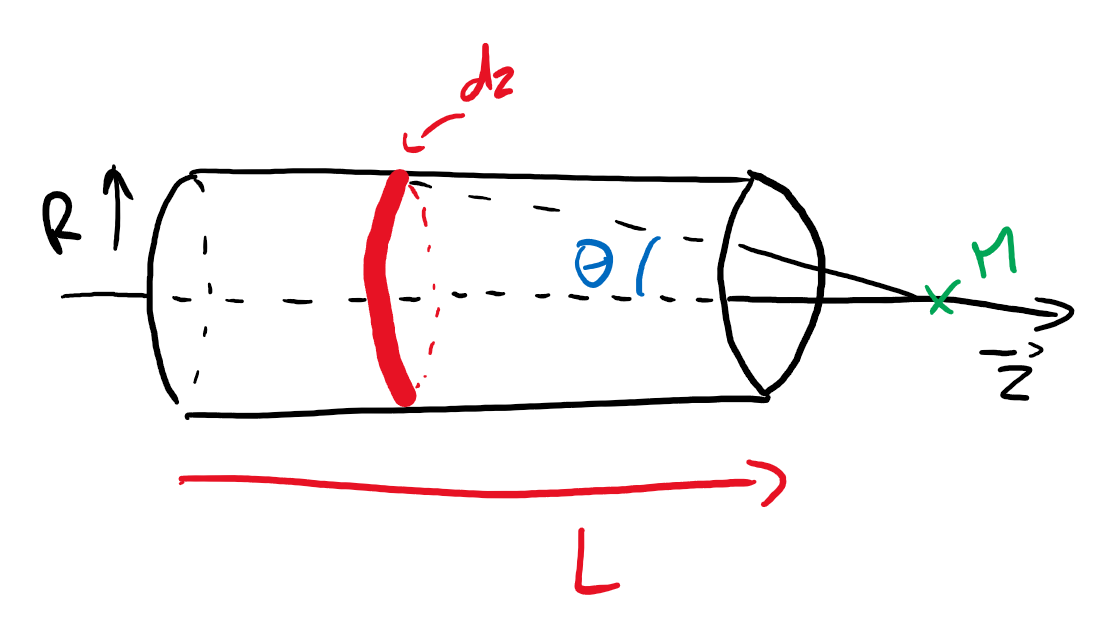
\includegraphics[scale=0.5]{solenoide_fini.PNG}
\end{figure}

$$\mathrm{d} \overset{\to}{B}(M) = n\mathrm{d}z\, \frac{\mu_0 I}{2 R} \sin^3(\theta) \overset{\to}{e_z}$$

\end{document}